\documentclass[fleqn,xcolor={usenames,dvipsnames},notes,aspectratio=169]{beamer} % [notes=only]
\usepackage{amsmath} % {amssymb,amsfonts}
\usepackage{eurosym}

% \usepackage{array,adjustbox} % url

% \usepackage{pifont,marvosym} % \ding

% \usepackage{multimedia}
% \usepackage[normalem]{ulem}
% \usepackage{framed,color,ragged2e}
% \usepackage[absolute,overlay]{textpos}
% \definecolor{shadecolor}{rgb}{0.8,0.8,0.8}

\usetheme{boxes}
\setbeamertemplate{navigation symbols}{}
% \useinnertheme{circles}

% Required by CAC
\setbeamercolor{background canvas}{bg=black!4}

\usepackage{xcolor}
\usepackage{tikz}
\usetikzlibrary{shapes,arrows}
\usetikzlibrary{tikzmark,positioning}
\usetikzlibrary{calc}

\newtheorem*{rawnamedtheorem}{\therawnamedtheorem}
\newcommand{\therawnamedtheorem}{\error}
\newenvironment{namedtheorem}[1]{\renewcommand{\therawnamedtheorem}{#1}
   \begin{rawnamedtheorem}}
  {\end{rawnamedtheorem}}


\title{Verifiable Luck}
% \subtitle{Verifiable random functions}


\author[Burdges]{Jeff Burdges}
\institute{
  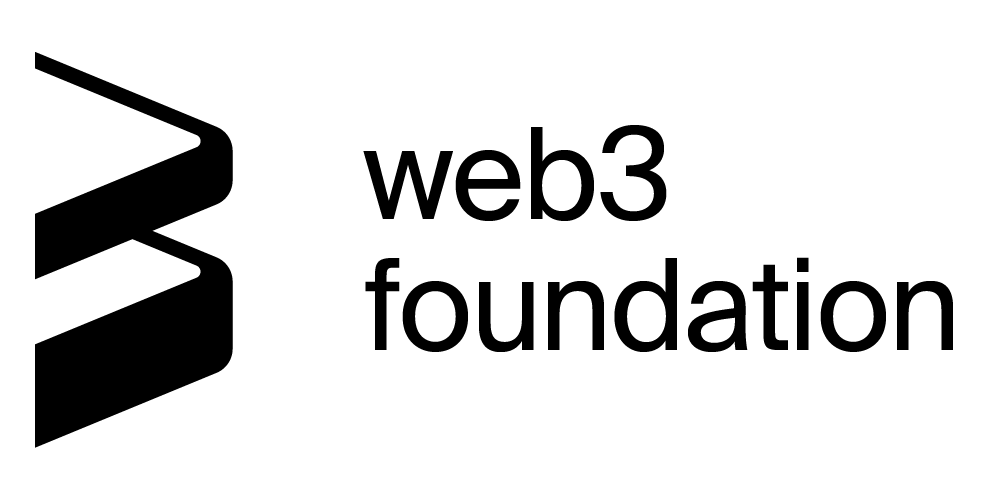
\includegraphics[scale=0.12]{../logos/Web3Foundation_2_2x.png}. % web 3 foundation
}
\date{15 Jan 2021} 

% \newcolumntype{R}[2]{%
%     >{\adjustbox{angle=#1,lap=\width-(#2)}\bgroup}%
%     l%
%     <{\egroup}%
% }
% \newcommand*\rot{\multicolumn{1}{R{45}{1em}}}% no optional argument here, please!

\def\signed #1 (#2){{\leavevmode\unskip\nobreak\hfil\penalty50\hskip2em
  \hbox{}\nobreak\hfil\normalfont --#1 (#2)%
  \parfillskip=0pt \finalhyphendemerits=0 \endgraf}}
% https://tex.stackexchange.com/questions/13756/quote-environment-with-reference-at-the-end-right



\newcommand{\algo}[1]{\ensuremath{\mathsf{#1}}}
\newcommand{\VRF}{\algo{VRF}} 
\newcommand{\RingVRF}{\algo{RingVRF}} 
\newcommand{\Sign}{\algo{Sign}} 
\newcommand{\Verify}{\algo{Verify}} 
\newcommand{\KeyGen}{\algo{KeyGen}}

\newcommand{\var}[1]{\ensuremath{\mathtt{#1}}}
\newcommand{\sk}{\var{sk}}
\newcommand{\pk}{\var{pk}}
\newcommand{\msg}{\var{msg}}
\newcommand{\aux}{\var{aux}}
\newcommand{\In}{\ensuremath{M}}
\newcommand{\PreOut}{\var{PreOut}}
\newcommand{\turnseed}{\var{turnseed}}

\newcommand\mdoubleplus{\mathbin{+\mkern-10mu+}}
\newcommand\concatvert{\mathbin\Vert}


\begin{document}


{\setbeamertemplate{footline}{}
\begin{frame}
\titlepage
\end{frame}
}
\setcounter{framenumber}{0}



\begin{frame}{What are VRFs?}

A verifiable random function (VRF) acts like a pseudo-random function (PRF) family, \\
\hspace*{10pt} but keyed by a public-secret key pair.  

\bigskip

VRFs weld a PRF into a signature scheme ($\KeyGen,\Verify,\Sign$) \\
\begin{itemize}
\item Uniqueness: $\VRF.\Verify_\pk(x,\sigma_1) = \VRF.\Verify_\pk(x,\sigma_2)$ unless either fail.
\item Pseudo-randomness: $F_\sk(x) = \VRF.\Verify_\pk( x, \VRF.\Sign_\sk(x) )$ is \\
\hspace*{10pt} hard to distinguish from a random function even with $\sk$, and \\
\hspace*{10pt} hard to compute without $\sk$. \\
\end{itemize}

\end{frame}



\begin{frame}{Instantiation}

\medskip

Naive RSA is deterministic, but \\
\hspace*{10pt} padding like PSS breaks uniqueness.

\medskip

RSA-FDH is both secure and deterministic, but \\
\hspace*{10pt} pseudorandomness needs $H(\sigma, \msg)$

\pause \bigskip \bigskip

Approach with elliptic curves : \\
\hspace*{10pt} Hash-to-curve $\In := H_1(\pk,\msg)$ \\
\hspace*{10pt} Prove correctness of $\PreOut := \sk \, \In$ \\
\hspace*{10pt} Return $H(\PreOut, \In)$ \\

\pause \bigskip
\hspace*{100pt}  {\bf BLS sucks !!!}

\end{frame}



\begin{frame}{Instantiation}

\medskip

Apply Fiat-Shamir to a $\sigma$-protocol:

\medskip 

\begin{columns}
\begin{column}[t]{0.05\textwidth}
\end{column}
\begin{column}[t]{0.475\textwidth}
    {\em $\Sign(\sk,\msg,\aux)$} \\
    \begin{itemize}
    \item $\In := H_1(\pk,\msg)$
    \item $\PreOut := \sk \, \In$
    \item $R := k (G + \In)$ with $k$ random
    \item $c := H_0(\In, \pk + \PreOut, R, \aux)$
    \item $s := k + c \, \sk$
    \item Return $\sigma = (\PreOut,s,R)$
    \end{itemize}
\end{column}
\begin{column}[t]{0.475\textwidth}
    {\em $\Verify(\pk,\msg,\aux,\sigma)$} \\
    \begin{itemize}
    \item $\In := H_1(\pk,\msg)$
    \item Check PoK on \pk, if needed
    \item $(\PreOut,s,R) := \sigma$
    \item $c := H_0(\In, \pk + \PreOut, R, \aux)$
    \item If $s (G + \In) = R + c \, (\pk + \PreOut)$ \\ then return $H(\In,\PreOut)$.
    \end{itemize}
\end{column}
\end{columns}

\bigskip

Resembles {V(X)Ed25519} by Perrin, IRTF draft by Goldberg, et al., \ldots

\end{frame}



\begin{frame} %{Verifiable card games}

\medskip

What are VRFs good for? \\
\hspace*{140pt} VRFs create an information asymmetry.

\bigskip\medskip

\begin{columns}
\begin{column}[t]{0.1\textwidth}
\end{column}
\begin{column}[t]{0.3\textwidth}
\includegraphics[width=.9\textwidth]{CAC/PNGs-to-print/individual-cards/black_FRONT026.png}
\end{column}
\begin{column}[t]{0.3\textwidth}
\includegraphics[width=.9\textwidth]{CAC/PNGs-to-print/individual-cards/white_FRONT085.png}
\end{column}
\begin{column}[t]{0.3\textwidth}
\includegraphics[width=.9\textwidth]{CAC/PNGs-to-print/individual-cards/white_FRONT126.png}
\end{column}
\end{columns}   

\end{frame}



\begin{frame}{Verifiably drawing cards}

% \medskip

As MPC is hard, our card deck has infinite repetitions on $n$ basic cards, \\
\hspace*{10pt} so no counting cards. 

\bigskip
\bigskip

{\em Rule:} All turns require a unique $\turnseed$ be unknown before the turn. \\ 

\bigskip

{\em Idea:} Player $\pk$ draws the cards given by $F_\sk(\turnseed \concatvert i) \mod n$, \\
\hspace*{10pt} where $F_\sk = \VRF.\Verify_\pk \circ \VRF.\Sign_\sk$ and $i=1 \ldots \var{numdraws}$.

\pause
\bigskip

Assume no collusion, next player gets $\turnseed := F_\sk(\turnseed \concatvert \texttt{"next"})$.

\bigskip

We prove draws and verify draw with our VRF \Sign\ and \Verify\ algorithms \\
\hspace*{10pt} by recording which player received which $\turnseed$.

\end{frame}



\begin{frame}

Signature semantics improve by signing more but.. \\ \smallskip
\hspace*{120pt}  VRFs are the opposite: less is more.

\bigskip\medskip

\begin{columns}
\begin{column}[t]{0.1\textwidth}
\end{column}
\begin{column}[t]{0.3\textwidth}
\includegraphics[width=.9\textwidth]{CAC/PNGs-to-print/individual-cards/black_FRONT050.png}
\end{column}
\begin{column}[t]{0.3\textwidth}
\includegraphics[width=.9\textwidth]{CAC/PNGs-to-print/individual-cards/black_FRONT012.png}
\end{column}
\begin{column}[t]{0.3\textwidth}
\includegraphics[width=.9\textwidth]{CAC/PNGs-to-print/individual-cards/white_FRONT227.png}
\end{column}
\end{columns}   

\bigskip\medskip

Our VRF inputs almost only $\turnseed$ ..

\end{frame}



\begin{frame}

Signature semantics improve by signing more but.. \\ \smallskip
\hspace*{120pt}  VRFs are the opposite: less is more.

\bigskip\medskip

Our VRF inputs almost only $\turnseed$ and \\
\hspace*{10pt} players reveal $\var{numdraws}$ before $\turnseed$. \\ \medskip 
 {\hfil $F_\sk(\turnseed \concatvert i) \mod n$ for $i=1 \ldots \var{numdraws}$ \hfil}

\bigskip

Think Crazy Eights, Mau Mau, or UNO, in which \\
\hspace*{20pt} our hand plus previous play determines $\var{numdraws}$!

% All draws occur during setup in Poker.

\pause
\bigskip
\bigskip
\bigskip
\textcolor[RGB]{220,220,220}{\rule{\linewidth}{0.2pt}}

An MPC looks not so much harder than addressing collusion. \\
\hspace*{20pt} Just shuffle! 

\end{frame}



\begin{frame}{NSEC5}

% \medskip

VRFs create an information asymmetry.. from a probabilistic algorithm.

\bigskip
\bigskip

DNSSEC needs authenticated responses for both record existence and non-existence,
\hspace*{20pt} but the authoritative server lives elsewhere. 

\bigskip

NSEC3 provides non-membership proofs for DNS zone records: \\
\begin{itemize}
\item Index zones by their hash
\item Authority signs adjacent hashed proving nothing lies in between
\end{itemize}

\bigskip

NSEC5 replaces NSEC3's hash with a VRF, \\
\hspace*{20pt} which prevents zone enumeration, even with rainbow tables!

\end{frame}



\begin{frame}{Go Fish}

\medskip

Go Fish players take action before draws: \\ \smallskip\smallskip
\begin{itemize}
\item Initially publish both $\pk$ and $\pk'$. \\ \smallskip
\item Reveal $\turnseed$ after naming victim. \\ \smallskip
\item Draw card face value with $\sk$ like above, \\ 
\hspace*{20pt}  $\var{card} := F_{\sk}(\turnseed) \mod n$. \\ \smallskip
\item Commit to cards and say ``Go Fish'' using $\sk'$, \\
\hspace*{20pt}  $\VRF.\Sign_{\sk'}( \var{card} \concatvert \var{replicate\_num} )$. \\ \smallskip
\end{itemize}

\end{frame}



\begin{frame}{Fog of War}

\medskip

{\em OpenConflict: Preventing Real Time Map Hacks in Online Games} \\
by Elie Bursztein, Mike Hamburg, Jocelyn Lagarenne, Dan Boneh.
Oakland 2011.
% https://crypto.stanford.edu/~dabo/pubs/papers/onlinegames.pdf

\bigskip

Uses Oblivious PRF, a similar MPC notion.  

\end{frame}



\begin{frame}{Polkadot games}

\begin{itemize}
% \item All players join $m$ equally sized teams, \\
%       make teams of size one for a more realistic game. \\
\item All $m$ players draw $k$ cards with repetitions, \\ 
      from an infinite deck with $n$ team cards. \\
\item All players socialize. 
\item All players have $k$ ``honest'' and ``cheat'' betting cards, \\
      with which they label each of their drawn team cards.
\item We reveal all face and betting cards: \\
\hspace*{5pt}  100\% ``honest'' teams' players get a point. \\
\hspace*{5pt}  100\% ``cheat'' teams' players win. \\
\hspace*{5pt}  Anyone cheating on a mix team looses. \\
\end{itemize}

\end{frame}



%\begin{frame}{Cover game}
%\end{frame}



\begin{frame}

We reveal information by not playing some cards..

\bigskip\medskip

\begin{columns}
\begin{column}[t]{0.1\textwidth}
\end{column}
\begin{column}[t]{0.3\textwidth}
\includegraphics[width=.9\textwidth]{CAC/PNGs-to-print/individual-cards/black_FRONT009.png}
\end{column}
\begin{column}[t]{0.3\textwidth}
\includegraphics[width=.9\textwidth]{CAC/PNGs-to-print/individual-cards/white_FRONT106.png}
\end{column}
\begin{column}[t]{0.3\textwidth}
\includegraphics[width=.9\textwidth]{CAC/PNGs-to-print/individual-cards/white_FRONT131.png}
\end{column}
\end{columns}   

\bigskip\medskip

We reveal cards' provenance when doing draw proofs, due to $\turnseed$ being public. \\ \smallskip
\pause
\hspace*{100pt} {\bf And reveals the player too!}

\end{frame}



\begin{frame}[t]{Anonymized signatures}

We know signatures that hide the signer:

\medskip

\hspace*{3pt} {\em Group signature:} Signer holds some bespoke certificate. \quad Efficient for pairings

\medskip

\hspace*{3pt}  {\em Ring signature:} Signer lies in a set specified by signer. % \quad $1$k Groth16, but set

\medskip

\hspace*{3pt}  {\em Linkable ring signatures:} Ring signature that reveals $\sk \, H_1(\textrm{"foo"})$

\pause
\bigskip
\bigskip

{\em Anonymized VRF:} Signer lies in \var{players}\ and reveal $\sk \, H_1(\pk,\msg)$

\medskip

$$ \algo{SNARK} \left\{ (\msg,\var{Out}) : \begin{aligned}
 &\var{Out} = H( \In, \sk \, \In ) \,\land \\
 &\In = H_1(\pk,\msg)  \,\land \\
 &\pk = \sk \, G \in \var{players} \\
\end{aligned} \right\} $$

\bigskip

Anonymized VRF plus Tor yields Verifiable Cards Against Cryptography! \\ 

\medskip

\end{frame}



\begin{frame}{Unethical Identity Systems I}

OpenID arguably makes sense for Stack Exchange, but.. \\
\hspace*{40pt}  Facebook Connect and Google Single Sign On pose a huge problem.

\bigskip

\begin{columns}
\begin{column}[t]{0.1\textwidth}
\end{column}
\begin{column}[t]{0.9\textwidth}

\includegraphics[width=.8\textwidth]{../pics/OpenID.jpeg}
\end{column}
\end{columns}

\end{frame}



\begin{frame}{Unethical Identity Systems II}

\medskip

W3C DID \& Verifiable Claims:  Users reveal certificates about themselves

\bigskip
\bigskip

What can go wrong? \\ \smallskip

\begin{itemize}
\item Discrimination 
\item Identity theft \\ \, \vdots
\item Details requested unnecessarily
\end{itemize}

\pause
\bigskip
\bigskip
\bigskip

% tl;dr \, All services gain equal consumers o

Can CL-signatures or similar help? \, Actually no.. \, Attributes cannot help.

\end{frame}



\begin{frame}{Ethical Identity Systems}

\medskip

{\em Assertion:} \, Services want users' identity to prevent Sybils \,\, -- Bryan Ford and others

\bigskip
\bigskip

Anonymized VRF output provide a unique identity for each domain:
\begin{itemize}
\item Identity request from $\texttt{domain}$.
\item Abort unless valid TLS certificate.
\item Abort unless user approves uniqueness to $\texttt{domain}$.
\item Return $\algo{AnonVRF}.\Sign(\texttt{domain})$
\end{itemize}

\bigskip

Actually used in Proof-of-Personhood Parties by Bryan Ford's DEDIS group.

\pause
\bigskip
\bigskip

Polkadot's future semi-anonymous single-leader election scheme for block production

\end{frame}



\end{document}




\begin{frame}
\end{frame}


\begin{frame}
\end{frame}












\begin{frame}

Zero-knowledge proof avoid revealing $\turnseed$ in its draw proof: \\ \smallskip

$$ \algo{SNARK} \left\{ (\pk,\var{Out}) : \begin{aligned}
 &\pk = \sk \, G \,\land \\
 &\var{Out} = H( \In, \sk \, \In ) \,\land \\
 &\In = H_1(\pk,\turnseed) \,\land \\
 &\turnseed \in \var{history}
\end{aligned} \right\} $$

\bigskip
\bigskip
And hiding the player looks easier: \\ \smallskip

$$ \algo{SNARK} \left\{ (\msg,\var{Out}) : \begin{aligned}
 &\pk = \sk \, G \in \var{players} \,\land \\
 &\var{Out} = H( \In, \sk \, \In ) \,\land \\
 &\In = H_1(\pk,\msg)  \\
\end{aligned} \right\} $$

\end{frame}



